 \chapter{ML-Agents Toolkit}\label{ml_unity}

% allgemeiner kram:
% https://github.com/Unity-Technologies/ml-agents/blob/master/docs/ML-Agents-Overview.md
% https://unity3d.com/de/how-to/unity-machine-learning-agents

In diesem Kapitel wird das Unity-Framework \Fachbegriff{ML-Agents} für die Entwicklung intelligenter Agenten auf der Grundlage von Reinforcement Learning vorgestellt. Der erste Abschnitt befasst sich mit einer Einleitung in die Unity-Engine. Anschließend werden der Aufbau und die Funktionsweise von ML-Agents skizziert und anhand einer Beispielimplementierung verdeutlicht. 

\section{Unity}
\Fachbegriff{Unity} ist eine State-of-the-Art Echtzeit-Entwicklungsplattform der Firma \Fachbegriff{Unity Technologies} für 3D-Simulationen und wird neben Teilbereichen wie Architektur und Industrie hauptsächlich für den Games-Bereich verwendet \cite{unity}. Zahlreiche Zielplattformen wie \Fachbegriff{Microsoft Windows} und diverse Spielekonsolen werden unterstützt. Unity liefert Features wie eine weit entwickelte Grafik- und Physik-Engine sowie einen modifizierbaren Editor für die Realisierung komplexer Projekte. Mit dem Editor können sämtliche gängigen Prozesse aus der Spieleentwicklung genutzt werden, beispielsweise aus den Bereichen \aufzaehlung{Networking} oder \aufzaehlung{Asset-Management}. Unity's eingebaute Mechanismen werden dabei durch Scripte ergänzt, um die Logik von Spielen zu implementieren. Abbildung \ref{fig:unity_heretic_demo} zeigt eine Momentaufnahme aus einer in Echtzeit berechneten Unity-Techdemo, um die Möglichkeiten der Engine zu verdeutlichen.

\begin{figure}[H]
\centering
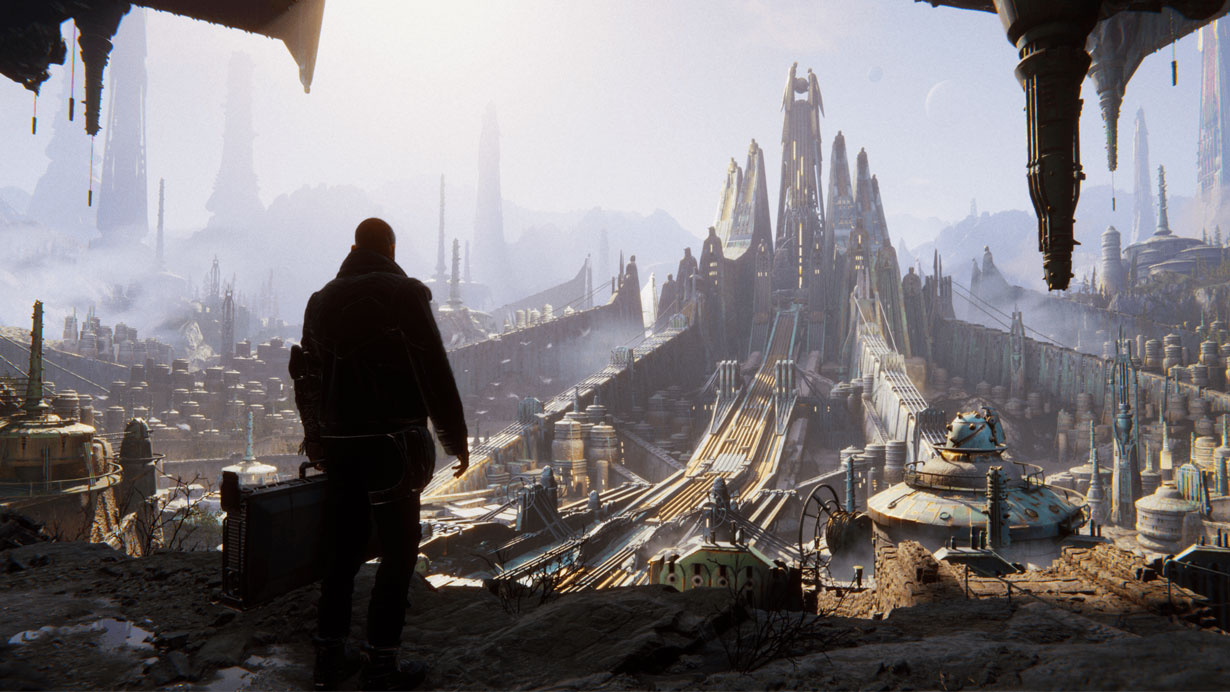
\includegraphics[scale=0.3]{images/ml-agents/unity_heretic_demo.jpg}
\caption{Unity-Echtzeitgrafik in \Fachbegriff{The Heretic} \cite{unity_heretic}}
\label{fig:unity_heretic_demo}
\end{figure}

Unity wendet sich sowohl an semiprofessionelle als auch hauptberufliche Spieleentwickler und große Entwicklerstudios. Mit einem Marktanteil von etwa 48\% im Vergleich zu den lediglich 13\% der \Fachbegriff{Unreal Engine} stellt sie die mit Abstand verbreiteteste Game Engine dar \cite{unity_marktanteil}.

\paragraph{Grundlagen}\label{scripting_unity_basics}
Unity verwendet die Programmiersprache C\# und erweitert diese um zusätzliche Konzepte, die speziell für die Entwicklung von Spielen vorgesehen sind. Alle in der Spielszene verwendeten Entitäten - unabhängig davon, ob sie über eine visuelle Repräsentation verfügen - basieren auf sogenannten \Fachbegriff{GameObjects}. Sie dienen als fundamentale Container, denen beliebig viele Komponenten hinzugefügt werden können. Scripts, die direkt an ein GameObject gebunden werden, heißen \Fachbegriff{MonoBehavior} und unterstützen eingebaute Funktionen der Engine wie beispielsweise die Funktion \inlinecode{Update}, die mit jedem neuen Frame aufgerufen wird. Komplexe hierarchische Konstrukte von \Fachbegriff{GameObjects} können anhand von sogenannten \Fachbegriff{Prefabs} zu Vorlagen transformiert werden, die auf der Festplatte gespeichert werden. Prefabs erlauben die Änderung von allen Objekten eines Typs durch die simple Anpassung des Basisobjekts. Weiterhin können große Mengen von Objekten desselben Typs leicht instantiiert werden.
Ein weiteres wichtiges Konzept sind \Fachbegriff{Coroutines}, welche in der Lage sind, die Ausführung einer Methode anzuhalten, um auf ein Ergebnis zu warten \cite{unity_coroutines}. Das geschieht mit dem Stichwort \Fachbegriff{yield}. Weiterhin können Coroutinen eigene Threads zugewiesen werden, indem \Fachbegriff{AsyncCoroutines} verwendet werden. Coroutines geben ein Ergebnis vom Typen \Fachbegriff{IEnumerator} zurück. Dieser Typ ist nicht Unity-basiert, sondern stammt aus dem \Fachbegriff{Microsoft .NET}-Framework. Coroutinen können nur von Monobehaviors durch die Funktion \Fachbegriff{StartCoroutine} und \Fachbegriff{StartCoroutineAsync} gestartet werden.


\paragraph{Unity Editor}
Unity liefert einen umfangreichen Editor für die Entwicklung von Spielen und Simulationen. Bis auf die Anfertigung von Assets und der Entwicklung von Programmcode finden alle Vorgänge zur Entwicklung eines Spiels in Unity selbst statt. Scripts werden in einer externen C\#-fähigen IDE entwickelt, wie zum Beispiel Visual Studio oder vergleichbaren Anwendungen. Ebenso werden Modelle und Grafiken in externen Anwendungen angefertigt.
Der Editor arbeitet szenenbasiert, wobei jede Szene ein eigenständiges Level darstellt. Im Verlauf dieser Arbeit wurde lediglich eine Szene für die Simulation des Dorfes entwickelt. Mit der Anwendung werden die folgenden Aufgaben bearbeitet:

\begin{itemize}
    \item Verwaltung eines komponentenbasierten Systems, Erzeugung und Manipulation von GameObjects 
    \item Bereitstellung einer Engine für physikalische Vorgänge wie Bewegungen, Kollisionen, etc.
    \item Rendering der Szene, Möglichkeit der Nutzung von Render-Pipelines
    \item Gestaltung des Levels mit visuellen Komponenten wie Mesh, Shadern, Texturen, Beleuchtung, Partikel, etc.
    \item Grundlegende Erzeugung und Manipulation weiterer Assets wie Sounds und Animationen (häufig in externen Programmen gelöst)
    \item Nutzung von Programmcode durch Scripts
    \item Verwaltung von Assets wie Sounds, Grafiken und 3D-Modellen
    \item Bereitstellung von speziellen Features wie Pathfinding und Leistungsoptimierungen wie \Fachbegriff{Occlusion Culling} \cite{unity_occlusion_culling}
    \item Bereitstellung diverser Plugins zur Erweiterung des Editors in beliebigen Bereichen
    \item Profiling und Debugging der Anwendung
    \item Ausspielen der Anwendung auf verschiedene Plattformen
\end{itemize}


Die Oberfläche des Editors wird in der Abbildung \ref{fig:unity_editor_overview} gezeigt. Das Bild zeigt die fundamentalen Komponenten des Editors.

\begin{figure}[H]
\centering
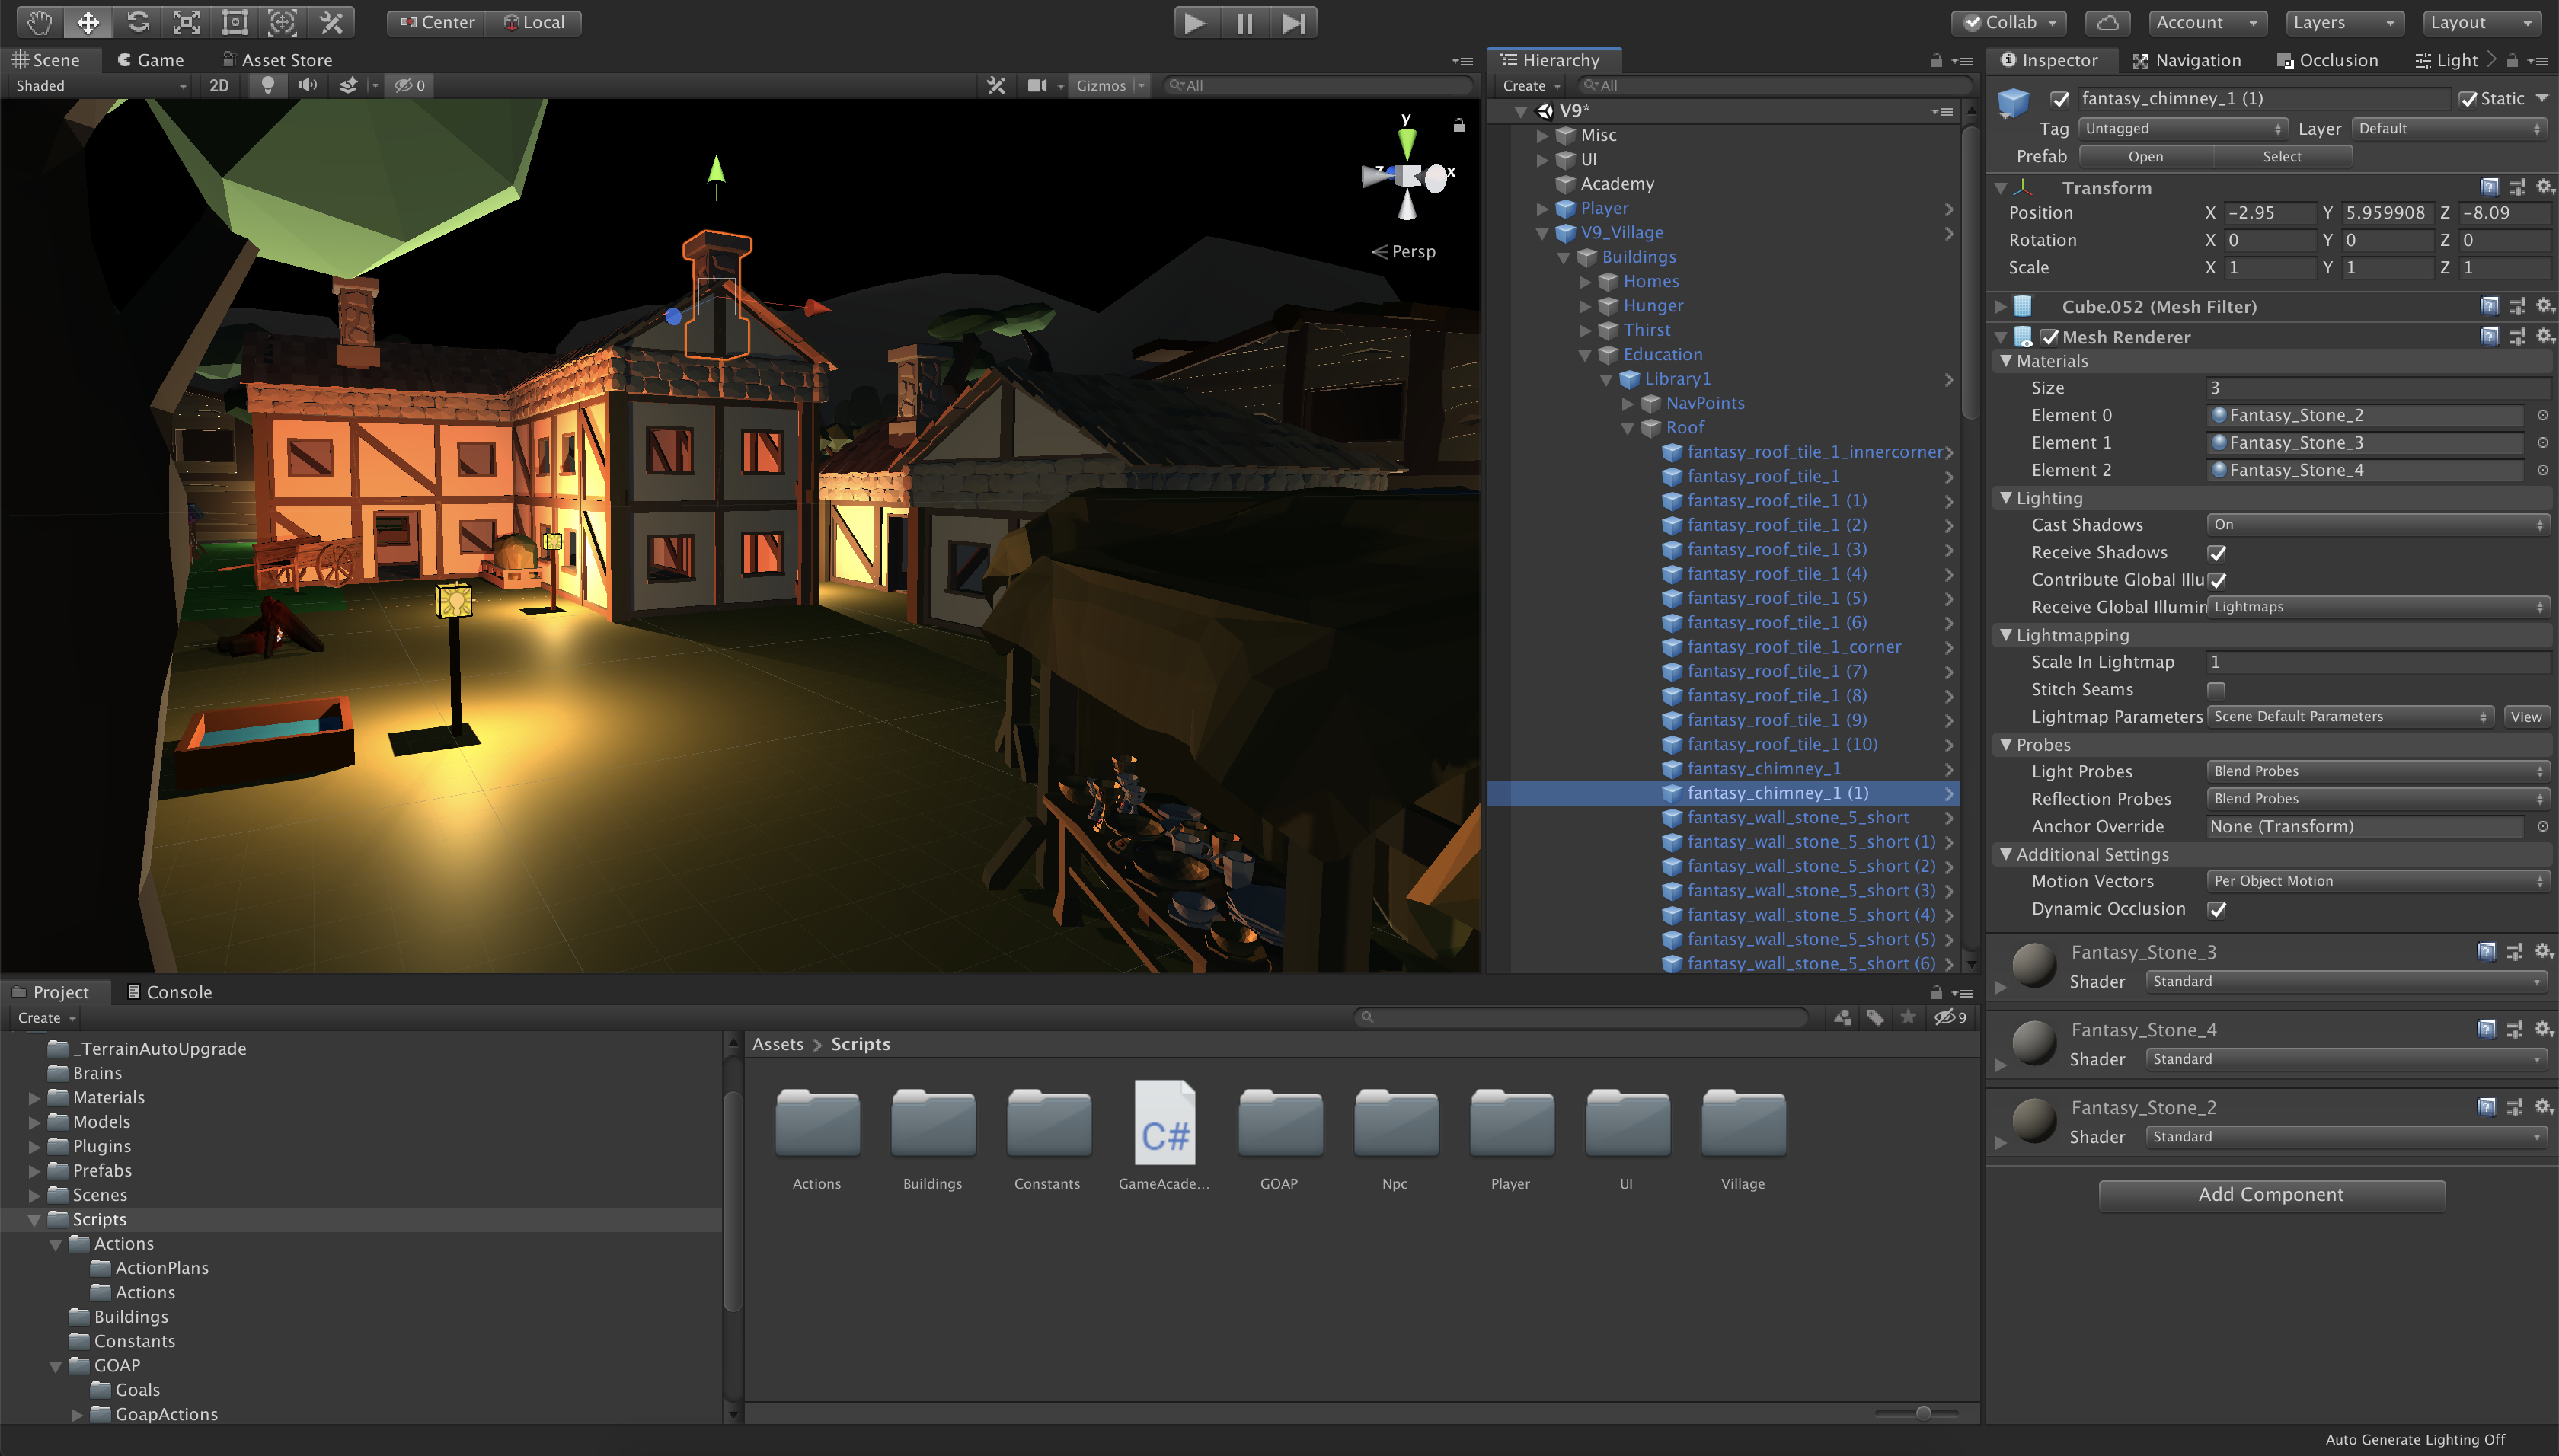
\includegraphics[scale=0.277]{images/ml-agents/unity_editor_overview.png}
\caption{Oberfläche des Unity Editors}
\label{fig:unity_editor_overview}
\end{figure}

Auf der rechten Seite ist der \Fachbegriff{Inspector} zu erkennen, der die Inspektion sowie das Hinzufügen und die Manipulation von Komponenten eines GameObjects erlaubt. Der Inspector zeigt die Komponenten des in der Szene ausgewählten GameObjects, die auf der linken Seite zu sehen ist und in der navigiert werden kann. In der Mitte der Abbildung ist die Szenenhierarchie zu erkennen, die den Aufbau der Szene beschreibt und Abhängkeiten von GameObjects definiert. Der untere Bereich zeigt die Ordnerstruktur des Projekts mit Assets, Scripts, Bibliotheken etc.
Ein großer Vorteil von Unity ist weiterhin die Möglichkeit, entwickelte Spiele direkt im Editor auszuführen, ohne dass Build-Vorgänge für spezifische Zielplattformen notwendig sind. Änderungen in der Szene oder im Programmcode können daher schnell getestet werden.



\subsection{Machine Learning in Unity}
Vor der Einführung von ML-Agents musste für die Nutzung von Machine Learning in Unity ein deutlich höherer Aufwand betrieben werden, da ausschließlich Community-Plugins verfügbar waren. Diese wurden sowohl genutzt, um eine Verbindung zu externen Schnittstellen wie Tensorflow aufzubauen, oder aber, um selbst neuronale Netzwerke zu implementieren. Da diese jedoch lediglich von Nutzern aus der Unity-Gemeinschaft entwickelt wurden, bestand aufgrund offensichtlicher Nachteile kein großes Interesse an der Verwendung von Machine Learning in Unity. Mit der Entwicklung des \Fachbegriff{ML-Agents Toolkit} wird der Einstieg in die Nutzung von Machine Learning in Unity extrem vereinfacht. Das Framework wird im folgenden Abschnitt näher skizziert.


\section{ML-Agents-Architektur}
\Fachbegriff{ML-Agents} ist ein von Unity Technologies entwickeltes Open-Source Framework, das Spielen und Simulationen erlaubt, als Entwicklungs- und Testumgebung für lernende Agenten zu fungieren \cite{ml-agents_paper} \cite{ml-agents_documentation} \cite{ml-agents_github}. Es befindet sich aktuell in der Beta-Phase, verfügt aber bereits über alle grundlegenden Features und ist öffentlich nutzbar. Mit ML-Agents wurde eine Plattform geschaffen, die die Entwicklung von lernenden Agenten einer größeren Menge von Entwicklern zugänglich machen, da sie vorhandene Hürden abbaut und den nötigen Aufwand reduziert.

In der Regel wird ML-Agents in der Kombination mit Imitation Learning oder Reinforcement Learning verwendet (siehe Abschnitte \ref{imitation_learning} und \ref{reinforcement_learning_intro}). Andere Verfahren wie genetische Algorithmen (z.B. \Fachbegriff{NeuroEvolution}), können ebenfalls verwendet werden, sind aber weniger gut dokumentiert und weniger üblich. Für den Trainingsvorgang stellt das Framework eine Verbindung zu einer Python-API her. Verschiedene State-Of-The-Art-Algorithmen wie \ac{ppo} und \ac{sac} werden dem Nutzer zur Verfügung gestellt. Das genaue Anwendungsszenario des Frameworks bleibt dabei dem Entwickler überlassen; es kann sowohl für die Verhaltenssimulation von NPCs als auch für automatisierte Tests oder der Evaluation des Game Designs verwendet werden \cite{ml-agents_github}. Ml-Agents bietet eine intuitive Architektur sowie eine große Menge von veränderbaren Parametern, um eine flexible Entwicklung von Agenten zu gewährleisten. Im Folgenden wird das Framework ausschließlich in der Kombination mit Reinforcement Learning verwendet.




\subsection{Grundlegende Funktionsweise}
Zur Installation wird ein \inlinecode{git clone} des ML-Agent GitHub-Archivs \cite{ml-agents_github} in ein leeres Unity-Projekt durchgeführt. Zusätzlich wird das \inlinecode{mlagents} Python Package benötigt. Diverse Beispiele sind bereits im Projekt enthalten und können zum Verständnis verwendet werden. Alternativ wird die Verwendung eines Docker-Image angeboten.

\begin{figure}[H]
\centering
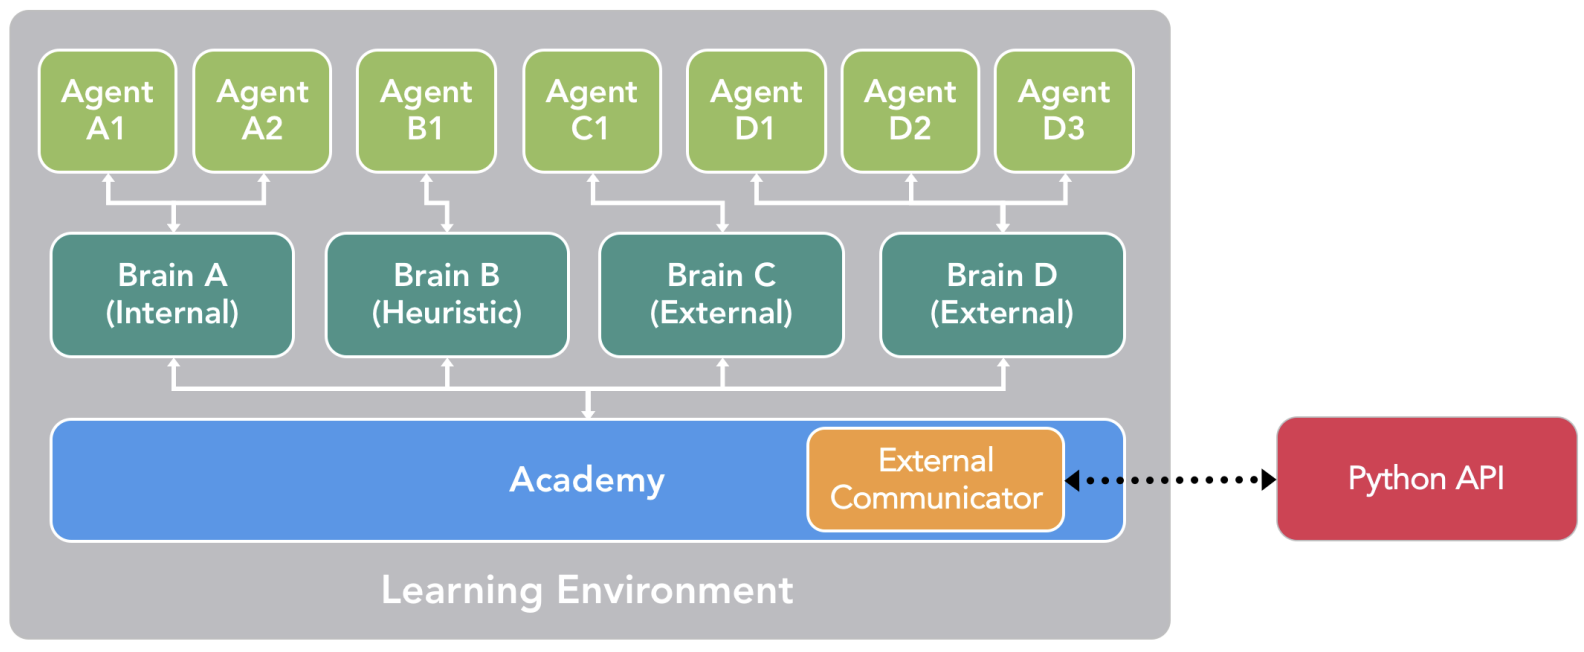
\includegraphics[scale=0.575]{images/ml-agents/architecture.png}
\caption{ML-Agents Architektur \cite{ml-agents_documentation}}
\label{fig:ml-agents_architecture}
\end{figure}

Vier grundlegende Klassen müssen in einem ML-Agents-Projekt verwendet werden, um einen lernenden intelligenten Agenten zu entwickeln. Im Einzelnen handelt es sich dabei um die folgenden zu implementierenden Konzepte, zu denen eine kurze Übersicht geliefert wird.

\newpage
\begin{itemize}
    \item \texttt{Agent}: Sammelt Observations und führt Aktionen aus.
    \item \texttt{Brain}: Das Gehirn der AI, trifft Entscheidungen.
    \item \texttt{Academy}: Zentrale Verwaltung aller Brains, externe Verbindung zu Python.
    \item \texttt{Model}: Resultat des Lernvorgangs, enthält Policy für ein Brain.
\end{itemize}

Die Abbildung \ref{fig:ml-agents_architecture} zeigt die zugrunde liegende Architektur, die die erwähnten Komponenten beinhaltet. Im Folgenden wird die Funktionsweise der einzelnen Konzepte beschrieben. Weiterhin wird näher darauf eingegangen, was bei einer Implementierung zu beachten ist.




\subsection{Academy}
Die Academy ist für die globale Koordinierung der Simulation zuständig. Sie dient als eine zentrale Verwaltungseinheit für alle Agenten und Brains. Durch die Herstellung der Verbindung zu einer externen Schnittstelle in Form eines Tensorflow-Backends stellt sie zusätzlich die Trainingsumgebung dar. Jegliche Machine Learning-Vorgänge sind vom eigentlichen Unity-Projekt völlständig entkoppelt, da der Entscheidungsprozess in Python abläuft.

Um Entscheidungen für Agenten zu treffen, findet eine kontinuierliche Kommunikation zwischen der Academy und der Python-API über den \Fachbegriff{External Communicator} statt (siehe Abbildung \ref{fig:ml-agents_architecture}), indem die Observations der Agenten an Tensorflow weitergeleitet werden. Tensorflow verfügt dabei über alle für das Training verwendeten Machine Learning-Algorithmen. Ein neuronales Netz innerhalb des Backends erzeugt einen Output, der die Entscheidung des Agenten in Abhängigkeit von den zuvor gesammelten Observations darstellt. Dieser Vorgang gilt sowohl für den Trainings- als auch für den Inference-Vorgang.

Zum Beginnn der Ausführung ruft die Academy die Funktion \inlinecode{AgentReset} für alle Agenten auf. Anschließend werden alternierend die Funktionen \inlinecode{CollectObservations} und \inlinecode{AgentAction} aufgerufen. Jeder Vorgang beinhaltet die Erzeugung einer Entscheidung durch das neuronale Netz und die Ausführung der entsprechenden Aktion durch den Agenten. Dies wird solange wiederholt, bis der Agent eine Episode abgeschlossen hat oder die maximale Schrittweite erreicht wurde. Anschließend wird der Prozess mit dem Aufruf von \inlinecode{AgentReset} erneut gestartet.

\subsection{Agent}
% https://github.com/Unity-Technologies/ml-agents/blob/master/docs/Learning-Environment-Design-Agents.md
Um einen neuen Agenten zu erzeugen, muss eine neue Klasse angelegt werden, die von der Oberklasse \Fachbegriff{Agent} erbt. Diese beschreibt die grundsätzlichen Aufgaben und nötigen Vorgänge eines lernenden Agenten. \Fachbegriff{Agent} erbt von der Unity-Basisklasse Monobehavior und verfügt daher über automatisch verwaltete Funktionen wie \Fachbegriff{Update} (siehe Abschnitt \ref{scripting_unity_basics}). Jeder Agent wird daher an ein GameObject angehängt. Folgende Funktionen müssen implementiert werden:

\newpage
\begin{itemize}
    \item \inlinecode{InitializeAgent}: Beinhaltet die einmalige Initialisierung des Agenten.
    \item \inlinecode{CollectObservations}: Vor jeder Aktion müssen Observations aus der Umgebung des Agenten gesammelt werden. Das können beispielsweise die Position des Agenten und eines Ziels oder dessen Lebenspunkte sein. Beobachtungen werden gesammelt, indem \inlinecode{AddVectorObs} aufgerufen wird. Diese Funktion unterstützt Zahlenwerte, Vektoren, Strings und Boolsche Werte. Weiterhin besteht die Möglichkeit, visuelle Beobachtungen zu verwenden. In dieser Arbeit wird diese Option nicht weiter behandelt.
    \item \inlinecode{AgentAction}: Die Parameter der Funktion beschreiben den Output des neuronalen Netzes. Der Agent muss entsprechend darauf reagieren und die jeweiligen Aktionen ausführen.
    \item \inlinecode{AgentReset}: Damit wird der Agent inklusive etwaiger Abhängigkeiten zurückgesetzt. Soll der Agent beispielsweise lernen, auf einer Plattform zu balancieren, so würde er beim Fallen von der Plattform wieder auf dieser platziert werden. Zusätzlich könnte die Plattform wieder horizontal ausgerichtet werden. \inlinecode{AgentReset} wird automatisch aufgerufen, wenn eine Episode endet, indem \inlinecode{Done} aufgerufen wird.
\end{itemize}

Essentiell sind die Funktionen \texttt{CollectObservations} für das Sammeln von Beobachtungen und \texttt{AgentAction}, um zu bestimmen, welche Aktion gewählt werden soll. Bei der Entscheidung der Aktionen kann zwischen zwei Szenarien gewählt werden. 

Bei den \Fachbegriff{diskreten} Entscheidungen wird anfangs eine Menge von möglichen Entscheidungen festgelegt, denen ein Index zugewiesen wird. In den Parametern von \inlinecode{AgentAction} wird dann ein einzelner Wert übermittelt, der eine ausgewählte spezifische Aktion referenziert, die ausgeführt werden soll. Der Output des neuronalen Netz bestimmt also die Ausführung einer bestimmten Aktion, indem ein ausgewählter Index für eine Aktion übermittelt wird. Diese Indizes werden durch Integer dargestellt, die bei $0$ aufsteigend beginnen.
Bei den \Fachbegriff{kontinuierlichen} Entscheidungen hingegen wird in jedem Fall für alle festgelegten Aktionen je ein Wert geliefert. Dabei werden keine Indizes, sondern skalare Werte anhand von Floats übermittelt, die die Amplitude für die jeweiligen Aktionen bestimmen. Diese haben einen Zahlenbereich von $-1$ bis $+1$. Ein mögliches Anwendungsszenario ist die Bewegung eines virtuellen Charakters. Es werden drei Aktionen festgelegt, um den Agenten erstens vor- und rückwärts und zweitens seitwärts zu bewegen. Die dritte Aktion bestimmt die Rotation des Agenten. Die Amplitude bestimmt nun, wie stark der Agent in eine Richtung bewegt oder gedreht werden soll, bzw. in welche Richtung er dabei vorgehen soll. Anstatt sich für eine Aktion zu entscheiden wird jeder möglichen Aktion also ein skalarer Wert zugewiesen, die den kontinuierlichen Ausschlag für die damit assoziierte Aktion bestimmt.


Eine essentielle Aufgabe des Agenten ist darüber hinaus die Erzeugung von Belohnungen. Die Funktion \inlinecode{AddReward} nimmt einen positiven oder negativen Float-Wert, der eine Belohnung oder eine Bestrafung darstellt. Es handelt sich also um einen skalaren Wert der beschreibt, wie gut der Agent agiert (siehe Kapitel \ref{reinforcement_learning}). Das mehrfache Aufrufen von \inlinecode{AddReward} führt zu einer Akkumulierung der Belohnungen. Außerdem besteht die Möglichkeit, den Reward direkt über \inlinecode{SetReward} festzulegen, wodurch bisherige Belohnungen für die ausgeführte Aktion ignoriert werden. Beim Training werden diese Belohnungen genutzt, um Beziehungen zwischen dem Spielzustand und den möglichen Aktionen herzustellen.

Zu Testzwecken können Entscheidungen vom Spieler selbst bestimmt werden. Dafür muss die Funktion \inlinecode{Heuristic} in der Agentenklasse überschrieben werden. Die Aktionen des Agenten werden dann nicht durch das Brain, sondern vom Spieler selbst bestimmt, indem den Aktionen Tastaturbefehle zugewiesen werden. Vor dem Training können so leicht Fehler entdeckt und die Funktionsweise eines Agenten getestet werden.

\subsection{Brain}
Zwischen der Academy und den Agenten existiert eine weitere zwischengeschaltete Entität namens \Fachbegriff{Brain}. Ein Brain kann beliebig viele Agenten verwalten (sieht Abbildung \ref{fig:ml-agents_architecture}). Jeder dieser Agenten verfügt über eine Referenz auf das Brain. Die Aufgabe des Brains ist die Bereitstellung einer Policy oder \Fachbegriff{Model} für alle mit ihm assoziierten Agenten und die Weiterleitung von Observations und Entscheidungen zwischen den Agenten und der Academy. Für jedes Brain wird im Tensorflow-Backend ein eigenes neuronales Netz angelegt.
Im Trainingsmodus werden für jedes Brain seperate Hyperparameter anhand einer Konfigurationsdatei zur Verfügung gestellt, die die Beschaffenheit des zugrunde liegenden neuronalen Netzes bestimmen. Jedes Brain wird außerdem über Parameter konfiguriert, die beispielsweise die Anzahl der Beobachtungen oder die Anzahl der möglichen Aktionen festlegen. Auch der Ablauf des Entscheidungsprozesses kann durch Parameter verändert werden: Standardmäßig wird nach einer festlegbaren Anzahl von Zeitschritten automatisch eine neue Entscheidung angefragt. Alternativ können sogenannte \Fachbegriff{On Demand Decisions} verwendet werden. Der Agent beantragt dann selbst eine neue Entscheidung, wenn seine vorherige Entscheidung abgeschlossen ist. Dies ist zum Beispiel nützlich, wenn die Dauer der Aktionen nicht absehbar ist.

\subsection{Model}
Beim \Fachbegriff{Model} handelt es sich um eine Policy bzw. ein Modell, das aus dem Trainingsvorgang eines Agenten hervorgegangen ist. Eine Policy ist nichts weiteres, als die Beschreibung der Parameter $\theta$ eines neuronalen Netzes, also der Gewichtungen der Neuronen. Für den Inference-Modus muss jedes verwendete Brain über ein \Fachbegriff{Model} verfügen. Ein Agent führt dann Aktionen aus, die das fertige Model aufgrund der Beobachtungen bereitstellt, ohne dass ein Trainings- oder Lernvorgang stattfindet.

Da die Parameter des Brains wie beispielsweise die Anzahl der Beobachtungen und möglichen Aktionen die Struktur des zugrunde liegenden neuronalen Netzes beeinflusst, ist das Model von ihnen abhängig. Sobald Parameter eines Brains verändert werden, kann ein trainiertes Model nicht mehr verwendet werden. In diesem Fall muss ein neuer Trainingsvorgang erfolgen.



\subsection{Training}
Während des Vorgangs versenden die Brains Observations der mit ihnen verknüpften Agenten über den External Communicator an die Python API und erhalten Aktionen als Antwort zurück. Innerhalb von Tensorflow findet dann der Lernprozess statt, in welchem die beste Policy für das jeweilige Brain gefunden wird. Nach dem Training wird das gelernte Model anhand einer Tensorflow Model-Datei mit der Endung \textit{.nn} gespeichert. Das Training kann sowohl mit nur einem als auch mit mehreren Agenten und Brains ablaufen. Die Verwendung mehrere Agenten kann die Geschwindigkeit und Stabilität des Trainings erhöhen \cite{ml-agents_documentation}. Für das Training werden die Framerate des Spiels und die Qualität der visuellen Darstellungen reduziert. Weiterhin kann die sogenannte \Fachbegriff{Time Scale} verändert werden, um schnellere Aktionen von den Agenten zu provozieren. Die in Unity eingebaute Time Scale simuliert eine Beschleunigung der Zeit. Sämtliche physikalische Aktionen laufen dann schneller ab. Update-Funktionen werden noch immer im selben Abstand aufgerufen, da sie entweder von der Framerate oder einem festen Intervall abhängen. Die scheinbar vergangene Zeit, die in Unity mithilfe von \inlinecode{Time.deltaTime} aufgerufen werden kann, erhöht sich dann proportional zum Time Scale-Faktor. 

Um einen Trainingsvorgang zu starten, können Befehle des \Fachbegriff{mlagents} Python Package verwendet werden. Diese sind unter \filepath{ml-agents/mlagents/trainers/learn.py} zu finden. Wichtig ist außerdem, dass in der Academy die zu trainierenden Brains referenziert werden und jeweils die Flag \Fachbegriff{Control} gesetzt wird. Folgende Anweisung wird verwendet, um das Training zu starten:

\begin{center}
    \inlinecode{mlagents-learn <config-file> --env=<env\_name> --run-id=<some-id> --train}
\end{center}

Der Parameter \inlinecode{env\_name} bezieht sich auf den Pfad der kompilierten ausführbaren Unity-Simulation. Wenn der Parameter nicht gesetzt wird, erfolgt das Training im Unity Editor. Nach dem Training kann mit dem Befehl \inlinecode{tensorboard --logdir=summaries --port <port-id>} ein \Fachbegriff{Tensorboard} verwendet werden. Ein lokaler Webserver wird dann gestartet, über den man in Echtzeit eine Visualisierung des Trainingsverlaufs betrachten kann. Über das Tensorboard können außerdem bereits vorhandene Trainingsdurchläufe evaluiert werden. In Abbildung \ref{fig:ml-agents_tensorboard} ist ein Tensorboard-Beispiel zu sehen. Zahlreiche Informationen zum Ablauf der jeweiligen Vorgänge stehen zur Verfügung. Dabei können anhand von Diagrammen Metriken wie die Belohnung, die Anzahl der Aktionen pro Episode, die Entropie der Policy und Weitere eingesehen werden.

\begin{figure}[H]
\centering
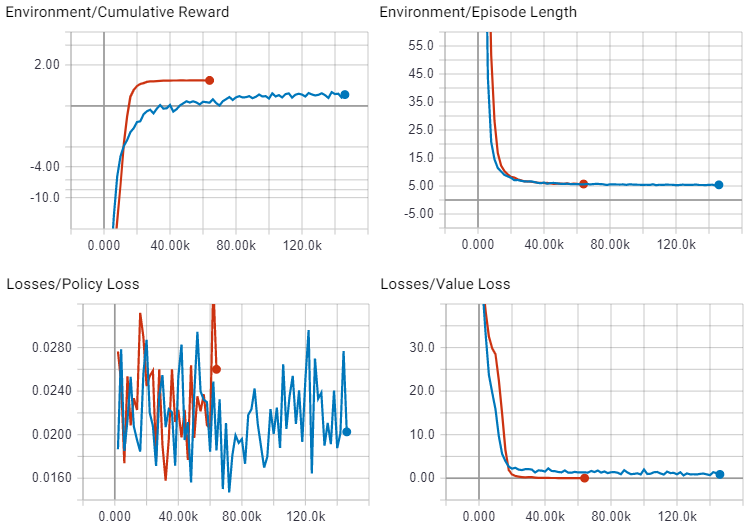
\includegraphics[scale=0.75]{images/ml-agents/tensorboard.png}
\caption{Tensorboard-Beispiel}
\label{fig:ml-agents_tensorboard}
\end{figure}

Weiterhin ist eine beispielhafte Konfigurationsdatei unter \filepath{config/trainer\_config.yaml} vorhanden. In dieser Konfiguration werden die Hyperparameter für das Training festgelegt. Dadurch kann unter anderem beschrieben werden, wie viele \Fachbegriff{Hidden Units}, also versteckte Neuronen, das neuronale Netz in wie vielen Schichten jeweils enthalten soll, oder auf welchen Wert die Lernrate festgelegt wird. Im Kapitel \ref{agenten_training} werden die einzelnen Hyperparameter näher beschrieben. Die Tabelle \ref{tab:ml-agents_training_hyperparameters} demonstriert eine Übersicht über die relevanten Parameter.
% advanced stuff???
    % curriculum: https://github.com/Unity-Technologies/ml-agents/blob/master/docs/Training-Curriculum-Learning.md
    % LSTM: https://github.com/Unity-Technologies/ml-agents/blob/master/docs/Feature-Memory.md
    % generalized agents for robust training: https://github.com/Unity-Technologies/ml-agents/blob/master/docs/Training-Generalized-Reinforcement-Learning-Agents.md




\section{ML-Agents-Beispiel}
Bei der Einarbeitung in das ML-Agents Toolkit wurde aus Gründen des Verständnisses und der Interesse ein Beispielprojekt angefertigt. Anhand dieses Beispiels soll ein erweitertes Verständnis über die Funktionsweise des Frameworks entstehen. Das Projekt wird im Folgenden vorgestellt. Der Quellcode für das Projekt kann im dazugehörigen GitHub-Repository betrachtet werden \cite{thesis_github_project}.


\subsection{Aufgabe}
Das Projekt beinhaltet einen einzelnen Agenten in Form eines Balls. Dieser soll lernen, sich zu einem Ziel (\Fachbegriff{Target}) zu bewegen. Sobald der Agent das Ziel erreicht, erhält der Agent eine Belohnung $r = 1$ und das Ziel wird zu einem anderen Ort bewegt. Sowohl Agent als auch Target befinden sich auf einer Plattform, von der der Agent herunterfallen kann. In diesem Fall bekommt der Agent eine hohe Bestrafung $r = -1$ und die Episode wird zurückgesetzt. Eine weitere Bestrafung $r = -0.1$ wird jedes Mal vergeben, wenn der Agent sich in die falsche Richtung bewegt. Die Abbildung \ref{fig:ml-agents_example_scene_single} zeigt den simplen Aufbau der Szene.

\begin{figure}[H]
\centering
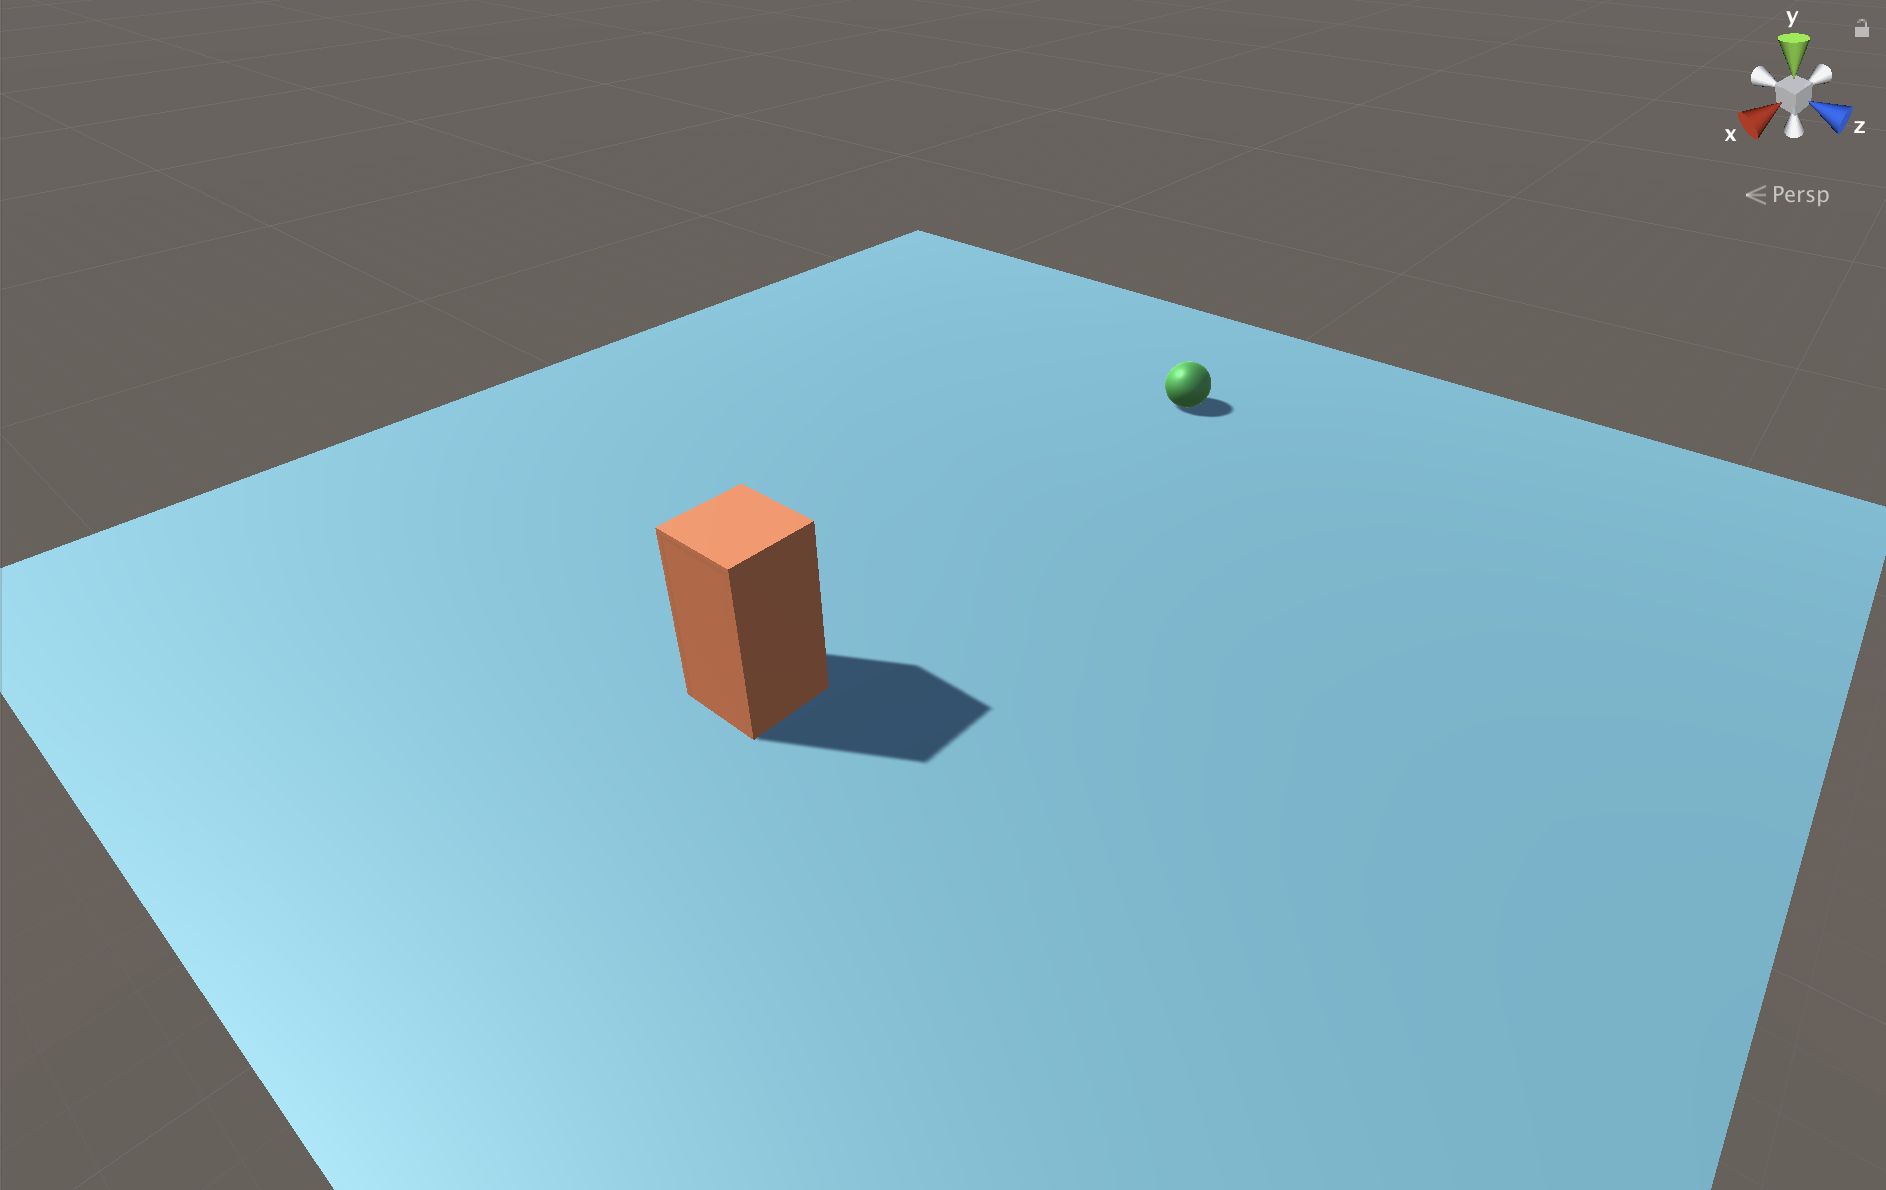
\includegraphics[scale=0.38]{images/ml-agents/example_scene_single.png}
\caption{ML-Agents-Beispiel, Aufbau der Szene}
\label{fig:ml-agents_example_scene_single}
\end{figure}


\subsection{Implementierung des Agenten}
Dieser Abschnitt zeigt, wie die einzelnen wichtigen Funktionen des Agenten implementiert wurden.

\paragraph{CollectObservations}
Das folgende Listing \ref{lst:ml-agents_example_observations} zeigt die Implementierung der Funktion \inlinecode{CollectObservations}. Die Wahl der Observations ist essentiell, damit sinnvolle Beziehungen zwischen Spielzustand und Belohnungswerten hergestellt werden können. Für die Lösung der Aufgabe sind vor allem die Position des Agenten und des Targets relevant, da der Agent sich darüber bewusst sein muss, in welche Richtung er sich bewegen muss (siehe Zeilen 3, 4, 8 und 9). Zusätzlich wird dafür die aktuelle Geschwindigkeit des Agenten verwendet. Diese wird von der \Fachbegriff{RigidBody}-Komponente bezogen, die GameObjects Interaktionen mit der Physik-Engine ermöglicht. Um Informationen darüber zu liefern, ob der Agent sich im Fallen befindet, wird weiterhin ein Boolscher Wert als Beobachtung hinzugenommen. Dadurch soll die Policy leichter eine Verbindung zu dem Grund der hohen erfahrenen Bestrafung erkennen können.

\begin{minipage}{\linewidth}
\begin{lstlisting}[linewidth=16.4cm, caption={ML-Agents-Beispiel, CollectObservations}, label=lst:ml-agents_example_observations, xleftmargin=1cm]
public override void CollectObservations() {
    AddVectorObs(this.transform.position.x);
    AddVectorObs(this.transform.position.z);
    AddVectorObs(_isAgentFalling());
    AddVectorObs(_agentRigidBody.velocity.x);
    AddVectorObs(_agentRigidBody.velocity.z);
    AddVectorObs(target.transform.x);
    AddVectorObs(target.transform.z);
}
\end{lstlisting}
\end{minipage}


\paragraph{AgentAction}
Zunächst wird ein Brain für den Agenten erstellt und konfiguriert, wie in Abbildung \ref{fig:ml-agents_example_brain_setup} erkennbar. Es soll ein kontinuierlicher Aktionsraum mit zwei Achsen verwendet werden, um den Agenten auf zwei Achsen zu bewegen. Für jede Aktion erhält der Agent dann zwei Werte, die seine Geschwindigkeit in X- und Z-Richtung beeinflussen. Weiterhin werden die in der Funktion \inlinecode{CollectObservation} getätigten Beobachtungen gezählt und eingetragen.

\begin{figure}[H]
\centering
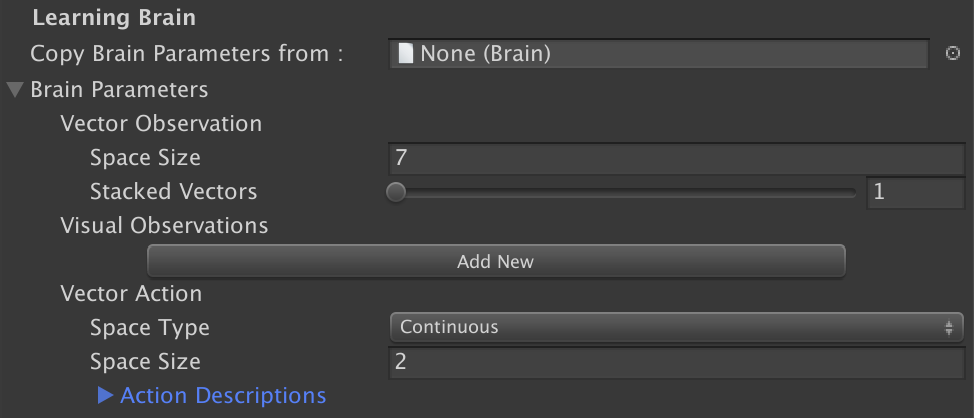
\includegraphics[scale=0.75]{images/ml-agents/example_brain_setup.png}
\caption{ML-Agents-Beispiel, Konfiguration des Brains}
\label{fig:ml-agents_example_brain_setup}
\end{figure}

Das folgende Listing \ref{lst:ml-agents_example_actions} zeigt die Aktionen, die der Agent ausführt, sowie die Verteilung der Belohnungen. Der Output des neuronalen Netzes wird in Form eines Float-Array zur Verfügung gestellt.

\begin{minipage}{\linewidth}
\begin{lstlisting}[linewidth=16.4cm, caption={ML-Agents-Beispiel, AgentAction}, label=lst:ml-agents_example_actions, xleftmargin=1cm]
public override void AgentAction(float[] vectorAction, string textAction) {
    // The agent fell off the edge. Finish episode with a punishment.
    if (_isAgentFalling()) {
        AddReward(-1f);
        Done();
        return;
    }
    // The agent has reached the target. Finish the episode with a reward.
    float currentDistance = Vector3.Distance(transform.position, target.transform.position);
    if (currentDistance < CLOSE_DISTANCE) {
        AddReward(1f);
        Done();
        return;
    }
    // Set the agents velocity to what the model thinks is a good value.
    float moveY = vectorAction[0] * SPEED_MULT;
    float moveX = vectorAction[1] * SPEED_MULT;
    _agentRigidBody.velocity = new Vector3(moveX, 0f, moveY);

    // In case the agent moved in the wrong direction, punish it.
    if (currentDistance > _lastDistance) AddReward(-0.1f); 
    _lastDistance = currentDistance;
}
\end{lstlisting}
\end{minipage}


\paragraph{AgentReset}
Weiterhin muss die Funktion \inlinecode{AgentReset} implementiert werden, um den Agenten und seine Umgebung zurückzusetzen (siehe Listing \ref{lst:ml-agents_example_reset}). Die Geschwindigkeit des Agenten wird zurückgesetzt und die Position des Targets auf der Plattform wird zufällig ausgewählt. Falls der Agent von der Plattform gefallen ist, wird auch dessen Position zufällig zurückgesetzt. Das Zurücksetzen der Positionen ist simpel, da die Plattform ihr Zentrum auf dem Koordinatennullpunkt besitzt. Dabei wird darauf geachtet, dass Agent und Target in einem gewissen Mindestabstand zueinander platziert werden.

\begin{minipage}{\linewidth}
\begin{lstlisting}[linewidth=16.4cm, caption={ML-Agents-Beispiel, AgentReset}, label=lst:ml-agents_example_reset, xleftmargin=1cm]
public override void AgentReset() {
    _agentRigidBody.velocity = _agentRigidBody.angularVelocity = Vector3.zero;
    if (_isAgentFalling()) _setRandomAgentPosition();
    _setRandomTargetPosition();
    _lastDistance = Vector3.Distance(transform.position, target.transform.position);
}
\end{lstlisting}
\end{minipage}


\paragraph{Multi Agent Training}
Um die Laufzeit des Trainings zu verringern, wurde ein \Fachbegriff{Multi-Agent-Training} verwendet. Mehrere Agenten lösen gleichzeitig die gleiche Aufgabe, sind aber in ihrem eigenen Umfeld gekapselt und interagieren nicht mit anderen Agenten oder Umgebungen. Durch die Anfertigung eines Prefabs, das das Spielfeld und den Agenten umgibt, kann dies sehr schnell realisiert werden. Geringfügige Änderungen des Codes sind dafür notwendig, die im GitHub-Repository eingesehen werden können. Beispielsweise muss ein Offset bei der Positionierung von Agenten und Targets sowie bei der Sammlung von Observations verwendet werden, das von ihren initialen Positionen abhängt. Der aktualisierte Aufbau der Szene ist in Abbildung \ref{fig:ml-agents_example_scene_multi} erkennbar.

\begin{figure}[H]
\centering
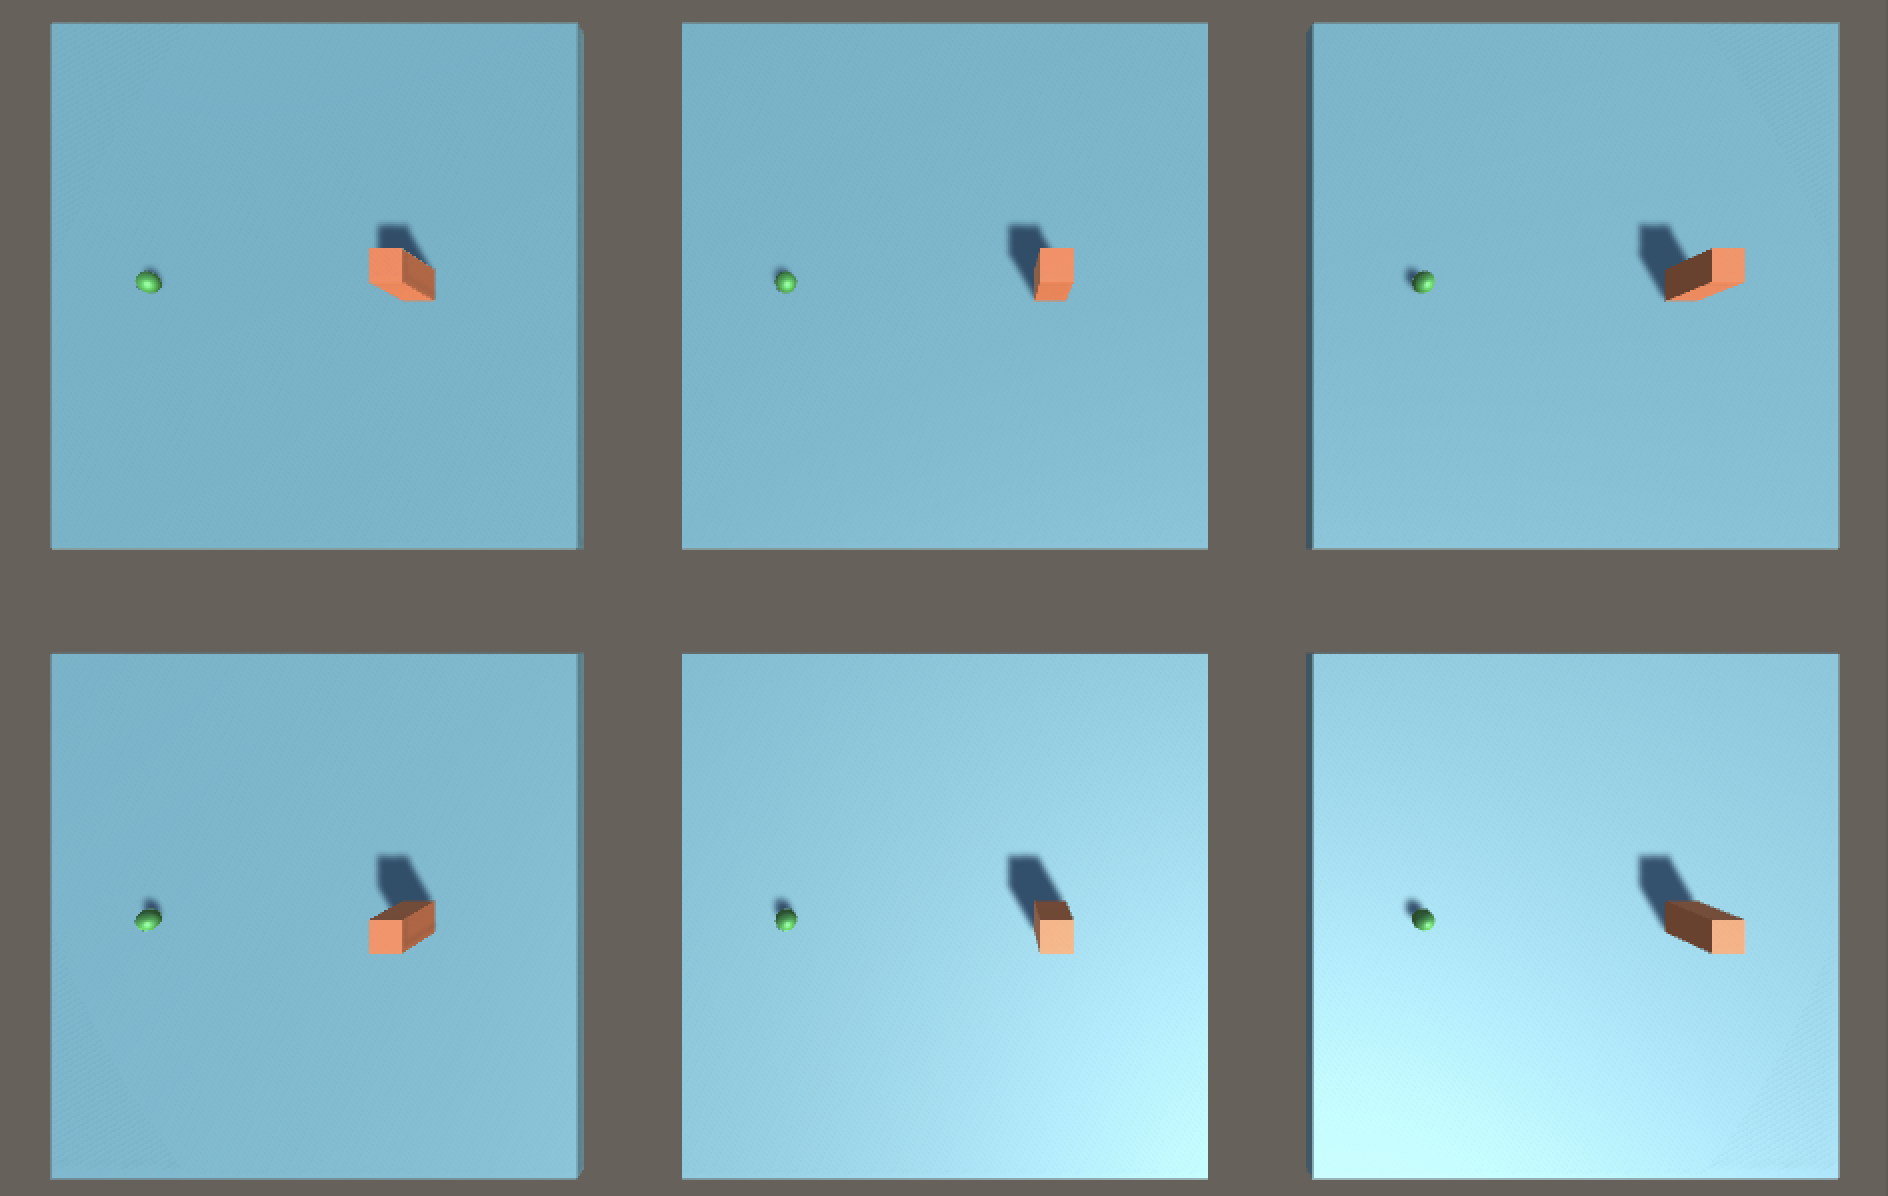
\includegraphics[scale=0.4]{images/ml-agents/example_scene_multi.png}
\caption{ML-Agents-Beispiel, aktualisierter Aufbau der Szene mit Multi-Agent-Setup}
\label{fig:ml-agents_example_scene_multi}
\end{figure}


\subsection{Training}
Das Training wurde mit \ac{ppo} und den Default-Hyperparametern durchgeführt, die um grob geschätzte Parameter erweitert wurden, die in der folgenden Auflistung zu finden sind. Die Funktionsweisen der einzelnen Hyperparameter werden im Abschnitt \ref{village_training_hyperparameter} ausführlich erläutert.

\begin{itemize}
    \item epsilon: 0.2, lambd: 0.95, beta: 3e-3, learning\_rate: 1e-3,
    \item num\_epoch: 3, max\_steps: 2e6
    \item use\_recurrent: false
    \item batch\_size: 1024, buffer\_size: 4096, time\_horizon: 32
    \item hidden\_units: 64, num\_layers: 2
    \item reward\_signals: extrinsic, strength: 1.0, gamma:0.99
\end{itemize}

Bei einem maximalen mathematisch möglichen Reward von $r = 1.0$ ergab sich bereits nach ca. 30.000 Schritten eine durchschnittliche Belohnung von $r = 0.94$ pro Episode. Nach etwa 45.000 Schritten wurde ein Wert von $r = 0.98$ erreicht und somit eine schnelle Konvergenz erreicht. Obwohl die Hyperparameter nur grob festgelegt wurden, wurde für diese einfache Aufgabe also nach kurzer Zeit ein gutes Ergebnis erzielt. Bezogen auf die kumulative Belohnung hat sich folgender Trainingsverlauf ergeben:

\begin{figure}[H]
\centering
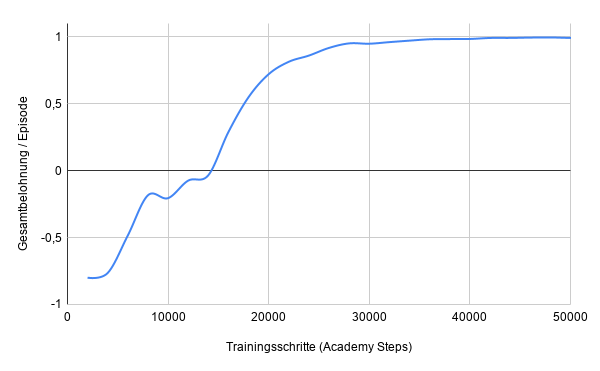
\includegraphics[scale=0.7]{images/ml-agents/diagram_example_training.png}
\caption{ML-Agents-Beispiel, kumulative Belohnung des Trainingsverlaufs}
\label{fig:ml-agents_example_training}
\end{figure}

In diesem Kapitel wurde bewiesen, dass einfache Vorgänge innerhalb kürzester Zeit gelernt werden können und dabei hohe Erfolgsquoten erreicht werden.
Im Folgenden wird auf dieser Erkenntnis aufgebaut und mit komplexeren Sachverhalten konfrontiert.